\documentclass[12pt]{article}
\setlength\parindent{0pt}
\usepackage{graphicx}
\usepackage[margin=1.0in]{geometry}
\usepackage{amsmath}
\usepackage{ulem}
\usepackage{color}
\usepackage{hyperref}
\setlength{\parindent}{2em}
\graphicspath{ {./images/} }
\title{CTA200H Assignment 2}
\author{Sarah Thiele}
\date{\today}

\begin{document}
\maketitle

\section{Question 1:}
\subsection{Methods}
This question studied the divergence of the magnitude-squared of the function 
\begin{align}
    z_{i+1}=z_i + c
\end{align} 
for numbers $c$ in the complex plane with real and imaginary parts $-2 \leq x,y \leq 2$. Here the magnitude, or absolute value, squared is defined as $|z_{i+1}|^2=(Re[z_{i+1}])^2+(Im[z_{i+1}])^2$. In order to work with every combination of $x$ and $y$ values, I defined 400-element arrays of each, and used numpy's function "meshgrid" which created a 2-dimensional array filled with the $x$ and $y\cdot i$ arrays. I then defined my complex array ``c" to be the sum of the zeroth and first dimension of the mesh such that we get a $400^2$ length array of the form $x+iy$. I arbitrarily defined an epsilon value of $\epsilon=100.0$ to use as a divergence measure, and a maximum iteration count of $i=1000$. We were given $z_0 = 0.0$. 

I next defined a function $recursion(c)$ which takes in the mesh c and uses a for loop to iterate Function (1). At each iteration, it takes the magnitude squared of the updated $z$ value, i.e $|z_{i+1}|^2$. If this value is greater than epsilon, then that element of the c array is said to be divergent. The function than adds the divergent values from that iteration to an array of divergent numbers, and adds the iteration number to another array the same number of times as the amount of divergent $z$ values there are for the iteration. e.g if three numbers diverge at iteration $i$, then those three numbers will be appended to the array defined as ``z\_div", and the iteration number $i$ will be appended three times to the array ``i\_div". This allows for every divergent element to have an iteration number associated with it when we plot the colour dimension, dependent on this quantity. The function then gets rid of values from the c array and the $z_i$ array which are divergent using a Boolean mask, and then moves on to the next iteration. Once we hit the maximum iteration number, the function defines all the remaining numbers to be those that remain bounded, and returns the arrays of bounded and divergent numbers as well as the iteration number array. We can then plot the complex plane with two colours defining the bound vs. divergent values, as we see in Figure 1, or with a colour scale which depends on the iteration number of divergence, like in Figure 2 and zoomed in version Figure 3, using matplotlib.

\begin{figure}
    \centering
    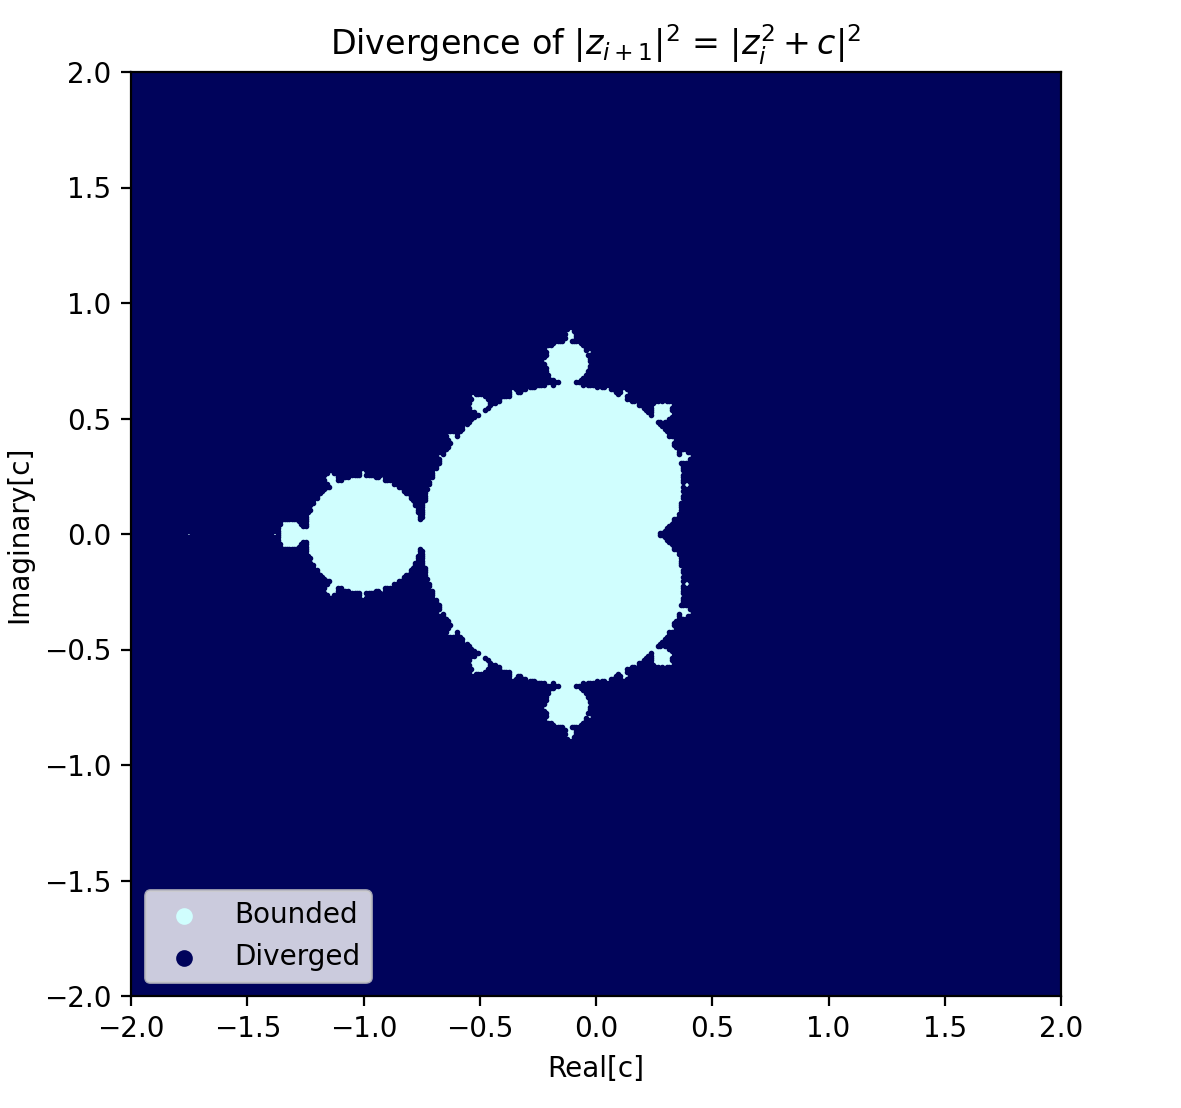
\includegraphics[scale=0.80]{Q1plot3_CITA200HA2.png}
    \caption{The divergence of complex magnitudes for $c = x + iy$ with $-2\leq x,y \leq 2$. The light blue region represents values that remain bounded, and the dark blue values diverge. Divergence was defined to be when $|z_{i+1}|^2 \geq 100.0$.}
    \label{fig:my_label}
\end{figure}

\begin{figure}
    \centering
    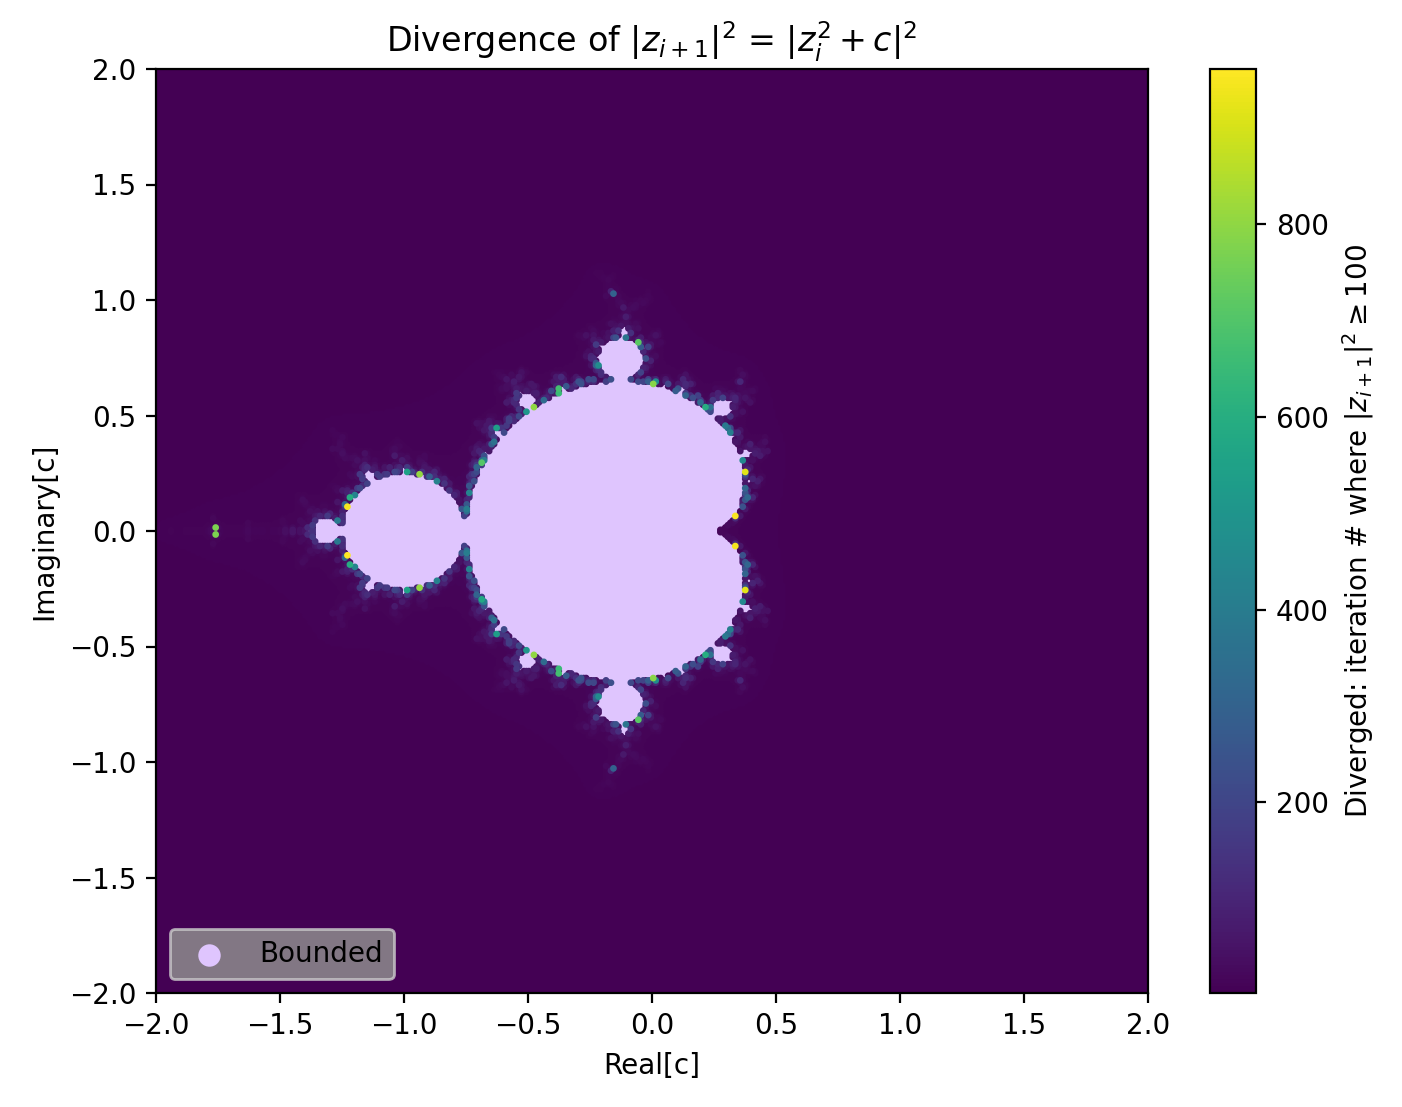
\includegraphics[scale=0.73]{Q1plot1_CITA200HA2.png}
    \caption{The same procedure as Figure 1, now coloured according to the value at which the number diverged, which is shown according to the colour bar. The light purple inner region again represents values which stay bounded.}
    \label{fig:my_label}
\end{figure}

\begin{figure}
    \centering
    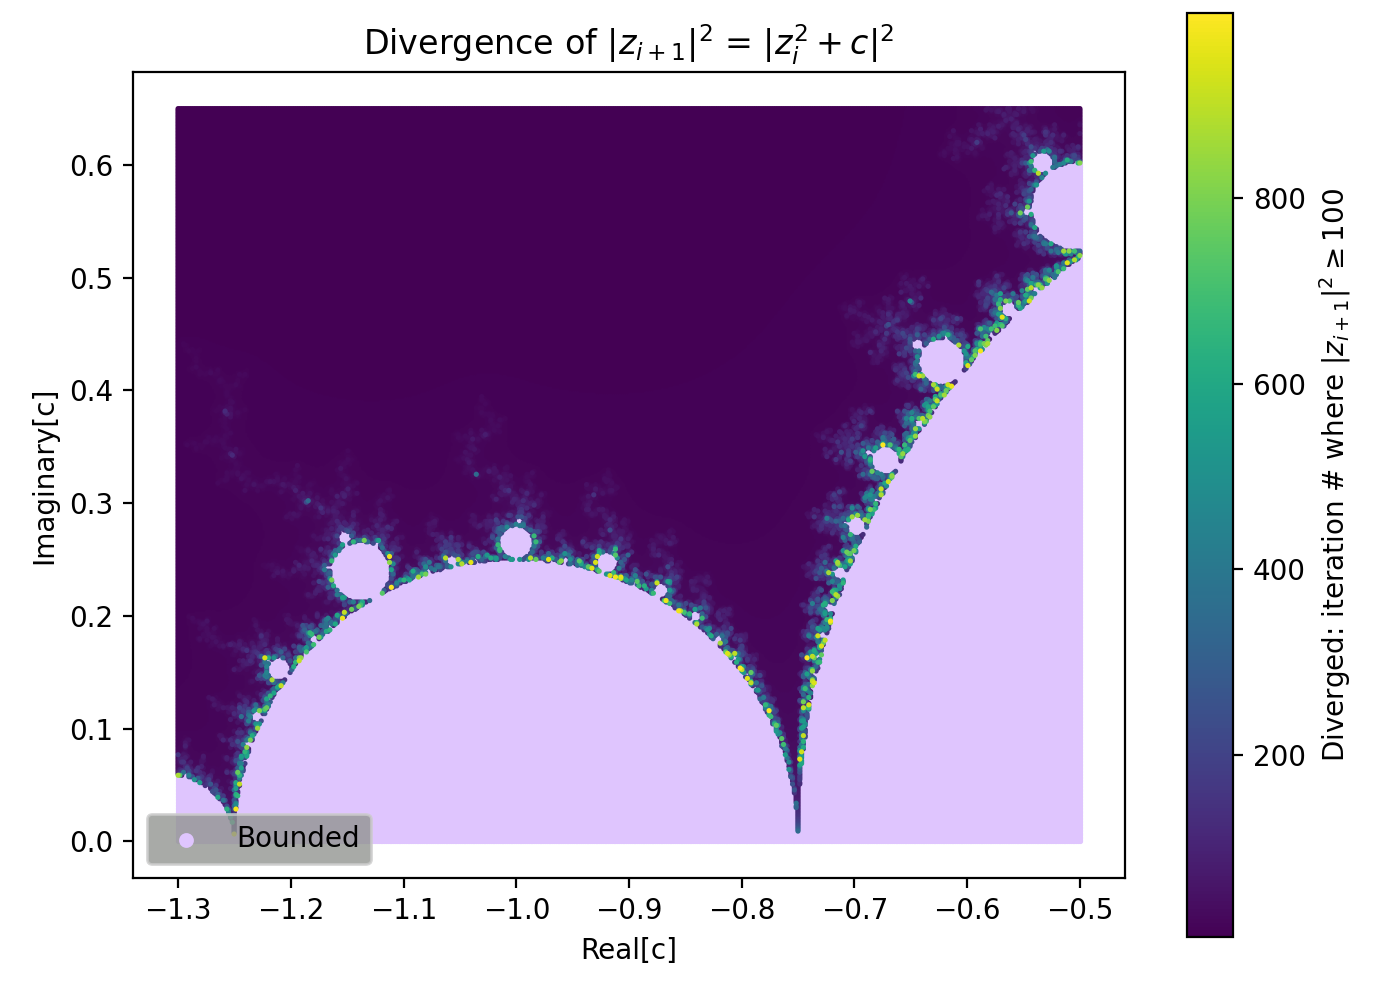
\includegraphics[scale=0.73]{Q1plot2_CITA200HA2.png}
    \caption{A closer look at our plot from Figure 2.}
    \label{fig:my_label}
\end{figure}

\pagebreak 
\subsection{Analysis}

What arises from the results of this question is the \href{https://en.wikipedia.org/wiki/Mandelbrot_set}{\color{blue}\uline{Mandelbrot Set}}, which would become increasingly intricate if we were to iterate with arrays of a smaller step size. Unfortunately, the computation time increases extremely fast for this function. We see that values closest to and on the boundary of the bounded region diverge much later than values further away from the bounded region. Outside the boundary, the values diverge almost immediately. We see that besides the main cardioid, the pattern is periodic with various sized circular bulbs. Furthermore the pattern is symmetric when flipped across the $x$-axis. When we zoom in, we can see there are small trails of slightly larger divergence iteration numbers that seep into the outer regions. These trails are lighter (diverge later) than those on the boundary. There is also a very faint tail that points straight leftwards from the smallest leftside bulb of the pattern and connects in a straight line to a small dot at ~(-1.75, 0.00). 

The zoomed-in plot had higher resolution, as it was along a smaller range of values ($-1.30 \leq x \leq -0.50$ and $0.00 \leq y \leq 0.65$), and the $x$ and $y$ arrays were each 600 elements in length. The faint trails are more pronounced and we can see some of the finer detail along the boundary.

\section{Question 2:}
\subsection{Methods}
\subsubsection{SIR Model}
In this question we were investigating the SIR Model in epidemeology which models the spread of disease for a given population. It is based on the following set of three ordinary differential equations:

\begin{align}
    \frac{dS}{dt} &= -\frac{\beta S I}{N} \\
    \frac{dI}{dt} &= \frac{\beta S I}{N} - \gamma I \\
    \frac{dR}{dt} &= \gamma I
\end{align}

As we can see, $\frac{dS}{dt} + \frac{dI}{dt} + \frac{dR}{dt} = 0$. Here $S(t)$ is the amount of the population susceptible to the disease and $I(t)$ is the number of infected individuals. In our homework it states that $R(t)$ is the number of recovered individuals who are now immune, but often $R(t)$ in the SIR model is simply the removed population, i.e those which are no longer susceptible or infected. It does not differentiate between those who are deceased and those that are recovered and now immune. For our purposes we will assume a death rate of 0\% such that $R(t)$ is the number of recovered individuals.

For the SIR Model, $\beta$ is the average number of contacts per person per time, i.e the infection rate, and $\gamma$ is often defined as $\frac{1}{T}$, where $T$ is the amount of time an individual is infectious for before an outcome occurs. N is the population number. 

The mathematical term $R_0$ to used to describe how contagious a disease is. It tells us how many people one individual will infect on average. It is also described with $R_0 = \frac{\beta}{\gamma}$. I chose $R_0 = 5$, and then calculated three values for $\beta$ from three values of $\gamma$ I chose from common ranges I saw online. We were also given initial values for S, I and R as 999, 1, and 0 respectively. The population number N is 1000.

To solve the system of ODEs, I used scipy.integrate's solve\_ivp. I first defined a model function which takes in a time array, a vector of S, I, and R for a particular time step, and the two parameters $\beta$ and $\gamma$. It calculates the current rate of change from the three equations and returns them in a list. For various values of $\beta$ and $\gamma$, solve\_ivp solves the system of ODEs for the defined time span of 0 to 200 and outputs a time array and the values of S, I, and R as a function of time. I then plotted the various curves.

\subsubsection{SIRD Model}

We now switch to the SIRD Model. S is again the number of people susceptible, and I those infected, to a disease as a function of time. The SIRD model is important as it differentiates the old R, the removed population from the SIR model, into either being recovered/immune (R) or deceased (D). $\beta$ is the infection rate, $\gamma$ is the recovery rate, and we add $\mu$, the now non-zero mortality rate. The ODEs change now to accommodate this: 

\begin{align}
    \frac{dS}{dt} &= - \frac{\beta S I}{N} \\
    \frac{dI}{dt} &= \left(\frac{\beta S}{N} - \gamma - \mu\right) \cdot I \\
    \frac{dR}{dt} &= \gamma I \\
    \frac{dD}{dt} &= \mu I
\end{align}

I assumed a mortality rate of 1\% and an initial death number of 0. The rest of the solution is the same as for the SIR Model, just with an extra ODE to solve. The other initial values, population number, and arrays for $\beta$ and $\gamma$ also remain the same. See \hyperref[subsec:AnalysisQ2]{\color{blue}\uline{here}} for analysis of Figure 4 and 5.

\begin{figure}
    \centering
    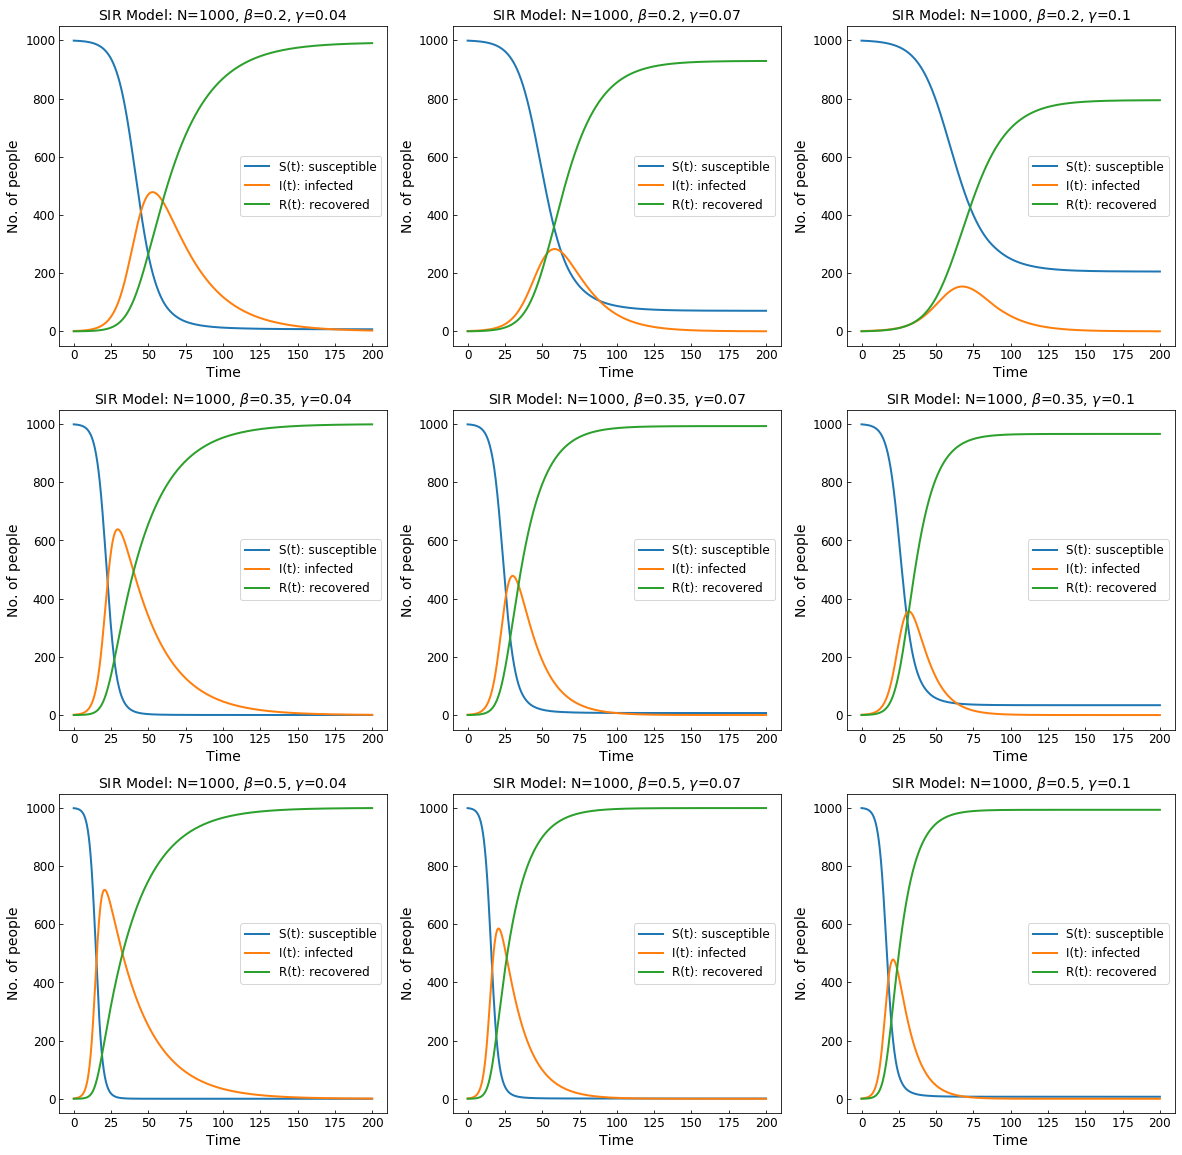
\includegraphics[scale=0.35]{SIR_Model_CTA200HQ2.png}
    \caption{Caption}
    \label{fig:my_label}
\end{figure}

\begin{figure}
    \centering
    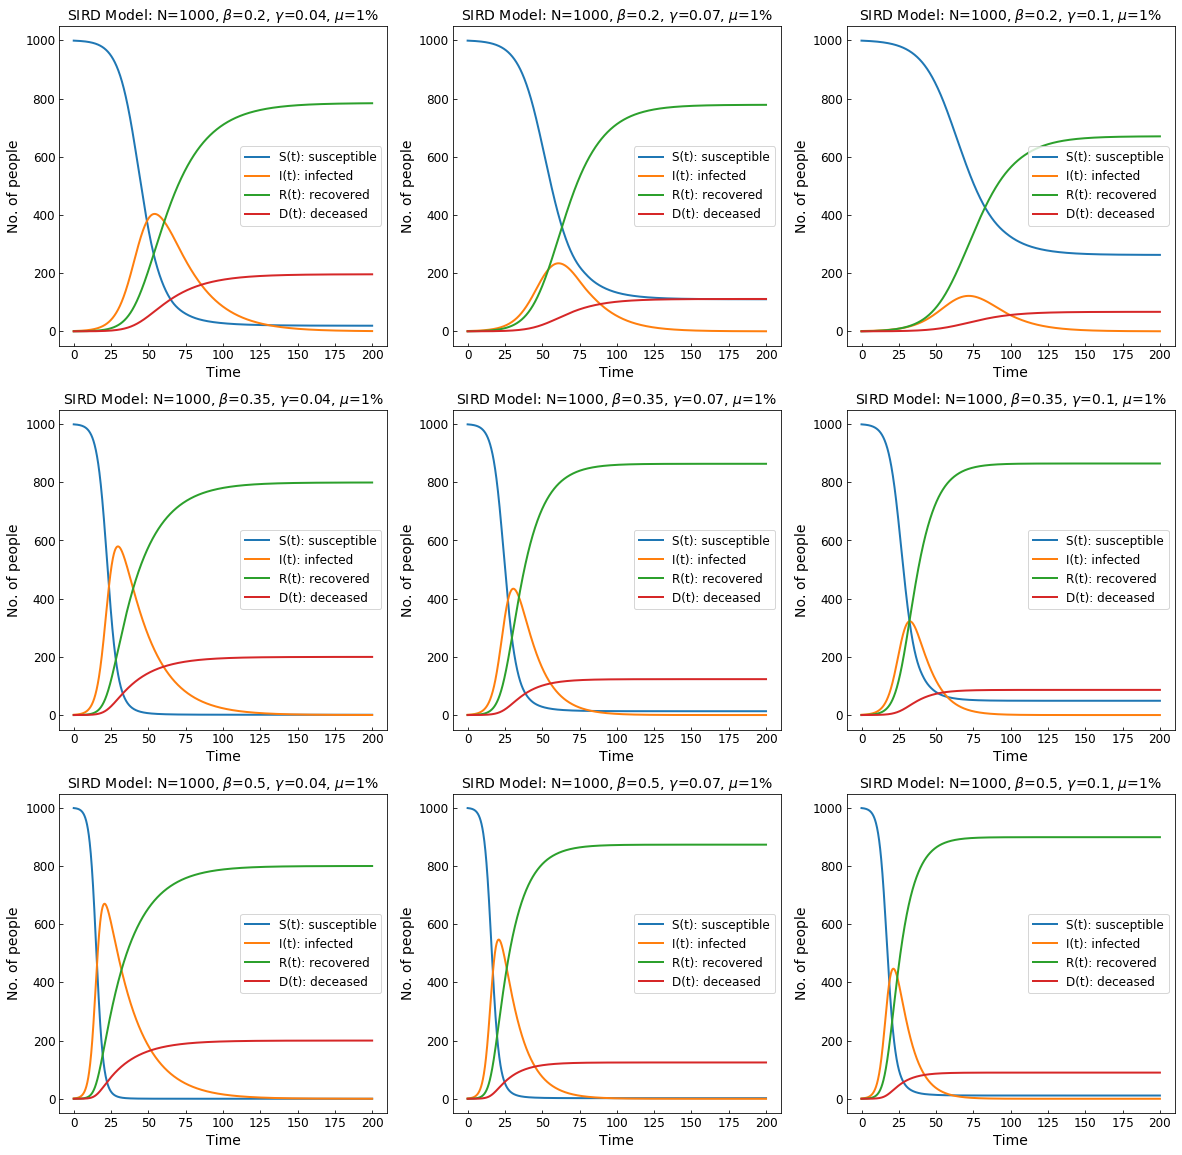
\includegraphics[scale=0.35]{SIRD_Model_CTA200HQ2.png}
    \caption{Caption}
    \label{fig:my_label}
\end{figure} 

\pagebreak

\subsection{Analysis}
\label{subsec:AnalysisQ2}

\subsubsection{SIR Model: Figure 4}
We see the expected general trends: the susceptible population decreases as people are moved into either the infected or recovered category over time; the number of infected individuals increases rapidly, and decreases quite quickly as well for our parameters, with the decline of infection mirrored by a steep incline in recovered, or in general removed, individuals; All three curves asymptotically approach a single value. We see that the peak of the number of infected individuals occurs at about the same time where the curves pertaining to the susceptible and recovered populations intersect. This makes sense intuitively: to the right of this peak, the number of removed individuals overtakes the number of susceptible and continues increasing, and so the number of infected individuals decreases as we move forward in time. To the left of the peak, the number of susceptible individuals is higher than those recovered, so there are more people able to become infected and hence the number of infected is increasing, creating this global maximum. 

The amplitude of the curves and their decay times depend on the $\beta$ and $\gamma$ values. For constant $\beta$, across a row in Figure 4, the amplitude of the peak of infection becomes lower, and not all individuals become infected for higher values of $\gamma$ over the investigated time span, such that the susceptible population curve does not reach zero. Since $\gamma$ is the inverse of the average time an individual is infected, a higher $\gamma$ means a fast recovery time, and so for constant infection rate this means the disease will be less aggressive but for a longer period of time. The decay rate of the curves, or their slope trend, remains similar across the figure's rows. For constant $\gamma$, down the figure columns, we see that the amplitude of the infection curve increases, as well as becomes steeper, i.e a smaller standard deviation. The slopes of the other curves also become much steeper. This is because for a constant recovery rate, an increase in the infection rate means that a disease will spread rapidly, hence the fast spike, and then decay as people recover. 

\subsection{SIRD Model: Figure 5}
For this model, we see the same trends as for the SIR Model. The only difference is that we now have a curve for the deceased individuals. It approaches a singular value which is a certain percentage of the population based on the mortality rate $\mu$ and the other parameters. The deceased curve increases faster for higher infection rates as expected. We also see the recovered line approach a lower value than for the previous model because not all individuals who's cases were resolved resulted in recovery - the disease also has a death rate now. 

We can interpret the two models as either that the SIR Model is working with a disease with a mortality rate $\mu=0$, and the SIRD model has $\mu \neq 0$, or that the SIR Model simply does not differentiate between recovered and deceased individuals. Either way, this explains the changes in amplitude of the recovered population. 

\end{document}